\subsection{Projeto de Software}

Em relação ao componente de software do projeto é necessário essencialmente reconhecer os comandos de voz feitos pelo usuário automaticamente, sem auxílio de palavras-chave ou de botões para acionar o sistema, recursos que costumam ser utilizados em outros projetos. Então o início do programa acontece ao identificar sinais no microfone em um volume mínimo pré-determinado. 
A partir desse instante o som começa a ser gravado, sendo que permanece desse modo durante alguns segundos. E após isso, o sinal de voz recebido será convertido para texto. Onde por fim, será analisado se alguma das palavras recebidas têm correspondência com a lista de comandos pré-determinados. Caso tenham, será realizada a função equivalente ao comando. E caso contrário, indicará que não houve palavra correspondente e voltará para o início do programa.
O algoritmo correspondente à essa parte está apresentado na Figura \ref{fig-DiagramaSoftware} a seguir. E utiliza-se do programa Julius para a decodificação e reconhecimento de voz.

\begin{figure}[htbp]
	\centering
		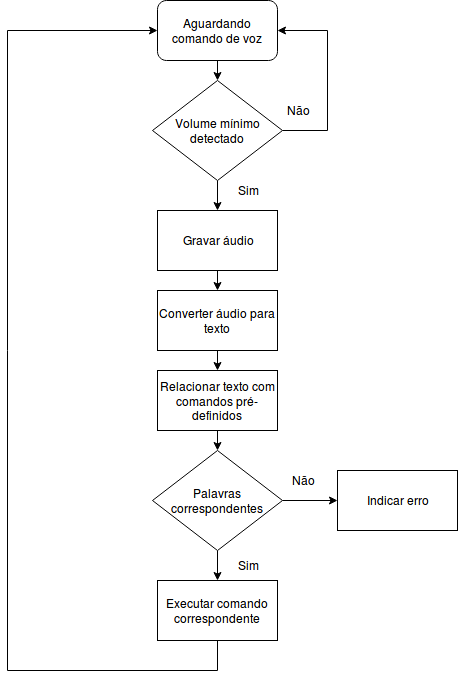
\includegraphics[scale=0.5]{DiagramaSoftware}
	\caption{Fluxograma do algoritmo}
	\label{fig-DiagramaSoftware}
\end{figure}

\subsubsection{Configurações necessárias}

Para o código funcionar da maneira correta foi necessário adaptar algumas configurações da raspberry pi e dos dispositivos tais como a webcam utilizada como microfone.
Então, para o reconhecimento de voz instalou-se a biblioteca libasound2-dev, o programa Julius e o pacote Quickstart-Linux.
E em relação ao microfone embutido na webcam Logitech c270 foi necessário checar por meio de diversos comandos se estava sendo reconhecido pela raspberry e funcionando da maneira correta.
O primeiro consistiu em "lsusb", para checar se o dispositivo aparecia na lista. Logo após,  utilizar o comando "alsamixer" a fim de aumentar o volume do microfone. Depois o "arecord -l" para testar se o microfone estava realmente sendo reconhecido.
E por fim, o "arecord -D plughw:1,0 test.wav" para gravar o som no arquivo test.wav, caso ao usar o comando "aplay test.wav" ouvir-se a gravação, o microfone está funcionando corretamente. 

\subsubsection{Programa Julius}

O Julius consiste em um programa com código aberto que é utilizado como decodificador para reconhecimento de fala. 
Foi desenvolvido sob os sistemas operacionais Windows e Linux. Possui amplo vocabuláio, alto desempenho e versatilidade. 
Sendo possível executar o reconhecimento de voz tanto em tempo real com dispositivos de entrada, quanto por meio de arquivos de áudio previamente armazenados nos formatos WAV.
Além disso, ele pode ser usado em conjunto com o software Coruja para adicionar a opção de reconhecimento de voz em português, tornando o programa mais acessível para os usuários.


\subsubsection{Funcionamento do código}

O programa ao ser executado procura pela entrada de áudio utilizada e o arquivo de configuração com extensão .jconf, local no qual são apontados quais devem ser os modelos acústicos e de linguagem a serem utilizados e o dicionário fonético que também é carregado. 
Se o carregamento de tais arquivos ocorrer sem erros, o programa Julius entra um laço de repetição, onde cada ciclo termina com o fim da entrada de áudio do usuário. Por fim, para cada comando dado pelo indivíduo, o programa reconhece se alguma das palavras ditas está entre as opções de palavras relacionadas aos comandos e realiza as ações associadas.  

\subsubsection{Resultados obtidos}

Com o código realizado até o momento, foi possível executar o programa "Rhythmbox" que é um player de música totalmente por meio de comandos de voz. 
Dentre as ações estabelecidas estão a execução do programa, tocar uma música, pausar, passar para a próxima ou retornar para a anterior.
De modo que para serem realizados estão entre as palavras de comando: play, next, previous, stop e show.


